\begin{tikzpicture}[]
    
 	\draw[->] (0,0)--(5,0) node[below,midway]{} node[below, midway, yshift = -0.5cm] {\small{$X$-tokens in LP}};	
 	\draw[->] (0,0)--(0,5) node[above,midway,rotate=90]{} node[above] {\small{$Y$-tokens in LP}};

	% Initial reserves
 	\draw[samples = 200, color=blue, scale=1, xshift = 0cm, yshift = 0cm, domain=0.9:4.55, smooth, variable=\x] plot ({\x}, {4/\x}) node[right, below] {\scriptsize{$k$}} ;    
    \draw[dotted, thick] (2,2)--(0,2) node[left]{\scriptsize 10};
    \draw[dotted, thick] (2,2)--(2,0) node[below]{\scriptsize 10};
	\draw[red, fill=red] (2,2) circle(1.2pt);

	% Delta x
	\only<2>{
		\draw[->, red] (2.05, 0.1) -- (2.95, 0.1) node [midway, above] {\scriptsize{5}};	
	}
	\only<2 | handout:0>{
		\draw[dotted,thick] (3,1.3) -- (3,0) node[below]{\scriptsize{15}};	
	}
	\uncover<3-5>{
		\draw[dotted,thick] (3,1.3) -- (3,0) node[below]{};
	}
	
	% Delta x minus fees
	\uncover<3-4>{
		\draw[dotted, red, thick] (2.8,1.43) -- (2.8,0) node[below]{\scriptsize{14}};

	}
	\uncover<3-4>{
		\draw[->, red] (2.95, 0.625) -- (2.85, 0.625) node {};	
	}
	
	% y'
	\uncover<4 | handout:0>{	
		\draw[dotted,thick] (2.8,1.43) -- (0,1.43) node[left]{\scriptsize{$7.1429$}};
	}
	
	% k'
	\uncover<5->{
		\draw[samples = 200, color=blue, scale=1, xshift = 0cm, yshift = 0cm, domain=0.97:4.55, smooth, variable=\x] plot ({\x}, {4.3/\x}) node[right, above] {\scriptsize{$k'_\rho$}};

		\draw[dotted,thick] (3,1.43) -- (0,1.43) node[left]{\scriptsize{$7.1429$}};
		\draw[dotted, red, thick] (2.8,1.43) -- (2.8,0) node[below]{};
		\draw[red, fill=red] (3,1.43) circle(1.2pt);
		\draw[->, blue] (4.63, 0.85) -- (4.63, 1.0) node {};		
	}	
	\uncover<5- | handout:0>{
		\draw[dotted,thick] (3,1.3) -- (3,0) node[below]{\scriptsize{15}};	
	}
\end{tikzpicture}